\chapter{Засоби формалізації голосової інформації в системах диспетчерського контролю за рухом автотранспорту} \label{chapt4}

\section{Особливості використання розроблених засобів формалізації голосової інформації в системах диспетчерського контролю за рухом автотранспорту} \label{sect4_1}

Для водія автомобілю, який буде здійснювати доставку продукції в процесі дистрибуції і вперше зіштовхнеться з засобом формалізації голосової інформації, що діє в рамках системи диспетчерського контролю за рухом автотранспорту, буде включений навчальний курс роботи з даною системою, в ході якого йому буде необхідно навчити дану систему розпізнавати його особистий голос з відповідними конкретними словами чи командами. Використання таких засобів формалізації голосової інформації на борту автомобіля дозволяє розширити швидкодію водія в процесі дистрибуції, забезпечити і підвищити рівень безпеки.

У даний час користувачі систем розпізнавання голосу змушені або працювати в умовах мінімального шумового фону, або використовувати мікрофонну гарнітуру. Що стосується того, щоб команда, випадково висловлена в слух водієм, не виконалась, у програму системи була додана функція пере запитування на виконання команди.

Інтерактивний інтерфейс в системі формалізації голосової інформації дозволяє водієві розмовляти з автомобілем (технічним засобом), створювати запити, отримувати інформацію і вказівки, вирішувати завдання з доставки продукції, у рамках системи диспетчерського контролю за рухом автотранспорту.

Сама точність розпізнавання мови водія багато в чому визначається якістю і стабільністю його вимови. Тому для попереднього навчання водіїв в голосовому інтерфейсі даної системи формалізації голосової інформації з диспетчерським контролем за рухом автотранспорту застосовується інформаційна система навчання. Виникаюче в них завдання постановки вимови, становить інтерес через велику сферу практичного застосування в різних областях. При цьому виникає проблема варіативності усного мовлення водіїв для різних носіїв національної мови і тісно пов’язана з нею проблема самостійної оцінки якості своєї вимови. У наявності очевидне протиріччя в самій постановці завдання: той, якого навчають з недостатньою на даний момент мовною підготовкою та обмеженими можливостями в процесі самонавчання повинен наблизитися за своєю вимовою до деякого еталону, який він слабо собі уявляє. Зазначене протиріччя з успіхом долається в запропонованій системі формалізації голосової інформації з диспетчерським контролем за рухом автотранспорту на основі критерію мінімуму інформаційного неузгодженості – на основі фонем. У цьому підході досяжність еталонної вимови забезпечується використанням не одного, а декількох «еталонів», які включають в себе і кращі зразки вимовлянь від одного або, навіть, декількох водіїв, які успішно пройшли навчання раніше. Така система формалізації голосової інформації здатна запам’ятовувати кращі вимови водієм слів і оцінювати якість подальшого виголошення тих же слів по відношенню до цих найкращих для водія словам, а не тільки по відношенню до використовуваних за замовчуванням стандартам, введених ідеальним водієм (диктором). При цьому у системі формалізації голосової інформації з диспетчерським контролем за рухом автотранспорту для оцінки якості вимови використовується тестування розрізнення різних звуків, яке може бути здійснено за допомогою одного з відомих методів автоматичного розпізнавання мови – пофонемного. У попередньому розділі показано, що для підвищення точності розпізнавання мови водія можуть бути застосовані ЗНМ.

При розробці систем розпізнавання дуже важливу роль грає експериментальний матеріал, на якому перевіряються і досліджуються запропоновані ідеї. В області розпізнавання мови в розробленій системі формалізації голосової інформації з диспетчерським контролем за рухом автотранспорту цей матеріал (слова і команди) є еталоном, який знаходиться в проміжній базі даних. По-іншому, таку базу даних можна позначити як корпус. Хоча корпуси усного мовлення вперше стали створювати для проведення фонетичних досліджень мови, широка потреба в них виникла, в значній мірі, завдяки розробкам в області автоматичного розпізнавання мови. На жаль, не існує універсальних мовних баз, які підійшли б для будь-якого завдання в області розпізнавання мови або фонетичних досліджень. Структура і склад мовного корпусу визначаються завданнями, які ставляться перед системою розпізнавання, яка використовує цей корпус.

У базі даних еталонів мовних фонем для систем голосового управління зібрано значну кількість необхідних прикладів виголошення заявлених для розпізнавання команд засобом формалізації голосової інформації в системах диспетчерського контролю за рухом автотранспорту.

Під час створення бази даних еталонів мовних фонем необхідно було вирішити чотири групи питань: технічні, змістовні, структурні та інструментальні (виконавчі).

Технічні питання пов’язані з вибором програмно-апаратних засобів запису мовного матеріалу (еталонів), а також з організацією необхідних умов запису, наприклад, виключення фонового шуму у засобах формалізації голосової інформації в системах диспетчерського контролю за рухом автотранспорту.

Змістовні питання в системі формалізації голосової інформації з диспетчерським контролем за рухом автотранспорту стосуються складу бази даних, а саме:

\begin{itemize}
	\item з вибором водіїв (дикторів) (кількість, стать, вік, діалектні відмінності тощо);
	\item з підбором текстового матеріалу (спеціалізований / репрезентативний, тип вимовлених мовних зразків (слова, команди, окремі пропозиції, тексти, зразки спонтанного мовлення), фонетично збалансований / незбалансований, тип балансування, статистичне представництво звукових одиниць тощо);
	\item з розподілом текстового матеріалу за водіями (дикторами), включаючи кількість підходів для кожного з них;
	\item з розподілом мовного матеріалу серед водіїв на тренувальну і тестову частини;
	\item з вибором типів інформації, яка асоціюється з кожним звуковим файлом (орфографічний запис, фонемний запис / фонетична транскрипція реального виголошення, акустико-фонетична розмітка звукового сигналу, інші типи анотацій і коментарів).
\end{itemize}

Структурні питання в системі формалізації голосової інформації з диспетчерським контролем за рухом автотранспорту визначають спосіб організації інформації, що міститься в базі даних еталонів, що пов’язані зі структурою директорій і файлів, зі створенням протоколів тощо.

До інструментальних питань в системі формалізації голосової інформації відносяться питання, що виникають у зв’язку з автоматизацією і стандартизацією різних етапів створення бази даних еталонів мовних фонем. При цьому в системі формалізації голосової інформації з диспетчерським контролем за рухом автотранспорту передбачені інструменти, що полегшують процеси транскрибування і структурування записаного матеріалу. Для цього у системі формалізації голосової інформації створена спеціальна програма, яка працює за методом суфлера (prompt-method). Дана програма дозволяє безпосередньо в процесі запису створювати звукові файли, що відповідають окремим об’єктам бази даних еталонів мовних фонем.

Як було зазначено вище, структуру і склад мовної бази системи формалізації голосової інформації з диспетчерським контролем за рухом автотранспорту визначають коло завдань, що вирішуються розробленою системою розпізнавання голосу.

У даній роботі при розробці засобів формалізації голосової інформації в системах диспетчерського контролю за рухом автотранспорту стояло завдання дослідити запропоновані методи розпізнавання слів (фонем) і їх реалізації в системі формалізації голосової інформації. Це дослідження можна провести на вирішенні задачі розпізнавання голосових команд. При такій спеціалізації програмного комплексу системи формалізації голосової інформації з диспетчерським контролем за рухом автотранспорту досягаються дві мети. По-перше, засіб розпізнавання голосових команд – центральний компонент системи формалізації голосової інформації, актуальність розробки якої позначена на початку даної роботи. По-друге, розширення завдання до розпізнавання злитого і спонтанного мовлення призвело б до невиправданого ускладнення програмного комплексу, викликаного необхідністю інтеграції СММ з лінгвістичної і іншими моделями мови.

Для проведення досліджень в рамках виконання дисертаційної роботи була складена власна база даних еталонів. Це було необхідно з наступних причин. По-перше, внаслідок специфіки розробляємої системи формалізації голосової інформації з диспетчерським контролем за рухом автотранспорту і завдань, які вона вирішує, знайти ідеально підходящу за структурою і складом базу даних еталонів мовних фонем неможливо; найбільш поширені бази даних (корпуси) з високою варіативністю звуків мови, що підійшло б для навчання і тестування систем розпізнавання спонтанної мови. По-друге, безкоштовних баз даних еталонів мовних фонем (корпусів) просто не існує. Нарешті, для наочності та усунення можливих лінгвістичних складнощів, найкращий був би корпус української або російської мови.

Склад створеної бази даних еталонів мовних фонем відповідає завданням, покладеним на систему формалізації голосової інформації з диспетчерським контролем за рухом автотранспорту. По-перше, кількість класів відповідає можливому числу і складу команд для розробленої системи голосового управління, включаючи числівники («один», «два», «перший», «другий» тощо), наприклад, для набору координат, і покажчики напрямку («прямо», «вправо», «вперед» тощо). По-друге, важливою рисою складеної бази даних еталонів мовних фонем є те, що усі навчальні і тестові приклади не перетинаються, що істотно підвищує достовірність результатів експериментальної перевірки системи формалізації голосової інформації. Процес побудови бази даних еталонів системи формалізації голосової інформації був автоматизований за допомогою розроблених програмних засобів попередньої обробки і поділу необхідних прикладів виголошення команд на окремі файли. Для об’єднання окремих етапів була використана скриптова мова та деякі засоби автоматизації \cite{tange_ole_2018_1146014}.

В ідеалі результатом розпізнавання фонем, що утворюють слово, як зазначалось, є його транскрипція, за якою слово в більшості випадків однозначно відновлюється. Однак, будь-які ознаки, що використовуються при розпізнаванні мови, мають характер випадкових величин. Тому на будь-якому етапі можлива відмова від розпізнавання і в результаті замість ланцюжка транскрипційних знаків на виході вийде послідовність символів, що позначають ті чи інші досить широкі класи фонем. Їх можна розглядати як результат змішання транскрипцій різного рівня деталізації. Виникає проблема, пов’язана з тим: як за таким різнорідним результатом у словнику команд (базі управління) відшукати необхідні слова, які йому задовольняють. 

У системі формалізації голосової інформації з диспетчерським контролем за рухом автотранспорту застосовано алгоритм, який дозволяє зробити це дуже швидко. Виграш в продуктивності став можливий завдяки структурі дерева сценаріїв, яке запропоновано в третьому розділі. Більш того, такий підхід виявляється корисним і в разі пошуку слів за узагальненою транскрипцією. Обхід дерева сценаріїв з підстановкою різних варіантів написання слова (фонеми) за узагальненою транскрипцією на кожному рівні дерева (тобто генерація варіантів написання слова за узагальненою транскрипцією в контексті вихідного словника команд для порівняння з навчальною вибіркою) скорочує значення M на кілька порядків.
Тобто кожен рівень дерева сценаріїв відповідає позиції контексту, що присутній у словнику команд (базі управління). Кожен вузол в рамках кожного рівня дерева є символ в слові відповідного контексту.

Для системи формалізації голосової інформації з диспетчерським контролем за рухом автотранспорту був розроблений засіб (додаток на мобільному пристрої) для збору голосових даних водіїв, експериментальні дані для якого наведені нижче.

\section{Апробація засобів формалізації голосової інформації в системах диспетчерського контролю за рухом автотранспорту} \label{sect4_2}

При здійсненні апробації засобів формалізації голосової інформації в системах диспетчерського контролю за рухом автотранспорту були зібрані наступні дані:

\begin{itemize}
	\item 4 пристрої, 23 диктори (11 жінок, 12 чоловіків), 94 варіанти стимулів (64 на основні реакції), 3046 зразків;
	\item  додатково 23 варіанти стимулів та 465 голосових зразків для реакції розпізнавання часу.
\end{itemize}

Розподілення дикторів при апробації засобів формалізації голосової інформації в системах диспетчерського контролю за рухом автотранспорту за пристроями приведено в таблиці \ref{tbl:data1_distribution}.

\begin{longtable}[c]{ | p{3cm} | p{3cm} | p{3cm} | p{3cm} | p{3cm} | }
	\longtableheader%
	{Розподілення дикторів при апробації засобів формалізації голосової інформації в системах диспетчерського контролю за рухом автотранспорту за пристроями}%
	{tbl:data1_distribution}%
	{Пристрій & Диктор & Стать & Кількість реакцій & Кількість стимулів}
	
	\multicolumn{5}{c|}{\todo{(Зробити таблицю розподілу)}}

\end{longtable}%


Проведене моделювання рефлекторними системами як у цілому так і за контекстами не дало результатів (табл. \ref{tbl:data1_irs13_total}, \ref{tbl:data1_irs24_total}). Моделювання нейронними мережами у цілому не дало результатів, а за контекстами дало певний результат – більше 50\%, але все-таки є достатньо низьким показником точності. Точність під час навчання, на навчальних даних досягала 100\%, що свідчить про перенавчання.

Покажемо графічно взаємовплив загальної кількості стимулів, розпізнаних стимулів та точністю розпізнання при апробації засобів формалізації голосової інформації в системах диспетчерського контролю за рухом автотранспорту (рис. \ref{img:data1_irs13_total}). Також для даних табл. \ref{tbl:data1_irs24_total} приведемо такий же розподіл на цьому ж рис. \ref{img:data1_irs24_total}.

\begin{longtable}[c]{ | >{\centering\arraybackslash}m{3.3cm} | >{\centering\arraybackslash}m{3.3cm} | >{\centering\arraybackslash}m{3.3cm} | >{\centering\arraybackslash}m{3.3cm} | }
	\longtableheader%
	{Відсоток розпізнавання за контекстами першого набору даних використовуючи ІРС з послідовностями розміром 1--3}%
	{tbl:data1_irs13_total}%
	{№ Контексту & Точність розпізнання & Кількість розпізнаних стимулів & Загальна кількість стимулів в контексті}	
	
	1 & 68.9 & 84 & 124 \\
	\hline
	2 & 45.6 & 234 & 513 \\
	\hline
	3 & 38.7 & 84 & 217 \\
	\hline
	4 & 37.5 & 39 & 104 \\
	\hline
	5 & 33.9 & 62 & 183 \\
	\hline
	6 & 39.7 & 83 & 209 \\
	\hline
	7 & 20.6 & 48 & 233 \\
	\hline
	8 & 34.6 & 75 & 217 \\
	\hline
	9 & 34.4 & 45 & 131 \\
	\hline
	10 & 34.9 & 44 & 126 \\
	\hline
	11 & 26.8 & 64 & 239 \\
	\hline
	12 & 26.4 & 53 & 201 \\
	\hline
	13 & 45.6 & 77 & 171 \\
	\hline
	14 & 43.9 & 61 & 139 \\
	\hline
	15 & 30.2 & 48 & 159 \\
	\hline
	16 & 47.8 & 55 & 115 \\
	\hline
	17 & 27.1 & 42 & 155 \\
	\hline
	18 & 41.8 & 46 & 110 \\
	\hline
	19 & 47.1 & 41 & 87 \\
	\hline
	По всій вибірці & 4.5 & 92 & 2069 \\
	\hline
	Тестовий контекст & 48.5 & 49 & 101 \\
\end{longtable}%

\begin{longtable}[c]{ | >{\centering\arraybackslash}m{3.3cm} | >{\centering\arraybackslash}m{3.3cm} | >{\centering\arraybackslash}m{3.3cm} | >{\centering\arraybackslash}m{3.3cm} | }
	\longtableheader%
	{Відсоток розпізнавання за контекстами першого набору даних використовуючи ІРС з послідовностями розміром 2--4}%
	{tbl:data1_irs24_total}%
	{№ Контексту & Точність розпізнання & Кількість розпізнаних стимулів & Загальна кількість стимулів в контексті}

	1 & 75.2 & 88 & 124 \\
	\hline
	2 & 89.8 & 459 & 513 \\
	\hline
	3 & 38.4 & 83 & 217 \\
	\hline
	4 & 55.8 & 58 & 104 \\
	\hline
	5 & 41.5 & 76 & 183 \\
	\hline
	6 & 56.5 & 118 & 209 \\
	\hline
	7 & 23.2 & 54 & 233 \\
	\hline
	8 & 37.3 & 81 & 217 \\
	\hline
	9 & 52.7 & 69 & 131 \\
	\hline
	10 & 53.2 & 67 & 126 \\
	\hline
	11 & 51.5 & 123 & 239 \\
	\hline
	12 & 48.8 & 98 & 201 \\
	\hline
	13 & 50.3 & 83 & 171 \\
	\hline
	14 & 63.3 & 88 & 139 \\
	\hline
	15 & 45.6 & 72 & 159 \\
	\hline
	16 & 58.3 & 67 & 115 \\
	\hline
	17 & 38.7 & 60 & 155 \\
	\hline
	18 & 58.2 & 64 & 110 \\
	\hline
	19 & 65.5 & 57 & 87 \\
	\hline
	По всій вибірці & 12.2 & 252 & 2069 \\
	\hline
	Тестовий контекст & 47.5 & 48 & 101 \\
\end{longtable}%

\begin{figure}
	\centering
	\subbottom[Розподіл за таблицею \ref{tbl:data1_irs13_total} \label{img:data1_irs13_total}]{%
		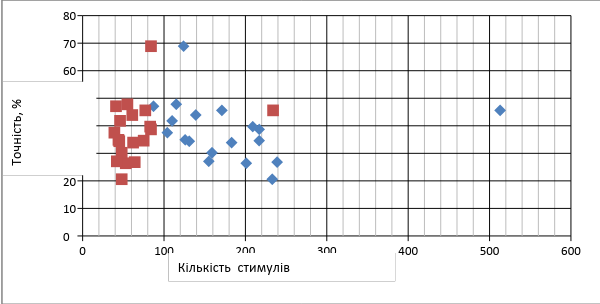
\includegraphics[width=\linewidth]{data1_irs13_total}}
	\\
	\subbottom[Розподіл за таблицею \ref{tbl:data1_irs24_total} \label{img:data1_irs24_total}]{%
		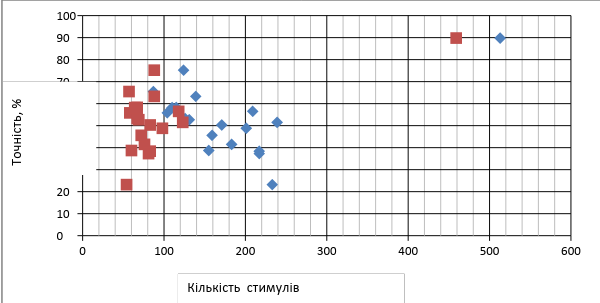
\includegraphics[width=\linewidth]{data1_irs24_total}}
	\caption{Розподіл точності розпізнання при відповідних стимулах: розпізнаних (червоні) та загальної кількості (сині) при апробації засобів формалізації голосової інформації в системах диспетчерського контролю за рухом автотранспорту для даних}
	\label{img:data1_irs}
\end{figure}

Була висунута гіпотеза про недостатню кількість вхідних даних. Були зібрані додаткові голосові дані для одного контексту: 1 пристрій, 1 диктор (чоловік), \todo{?} варіантів стимулів, 3 реакції у контексті, 938 зразків (табл. \ref{tbl:data2_irs13_total}, \ref{tbl:data2_irs24_total}).

Моделювання рефлекторними системами для одного контексту з великою вибіркою даних дало менше 70\% точності. Моделювання нейронною мережею дало більше 90\%.

\begin{longtable}[c]{ | >{\centering\arraybackslash}m{3.3cm} | >{\centering\arraybackslash}m{3.3cm} | >{\centering\arraybackslash}m{3.3cm} | >{\centering\arraybackslash}m{3.3cm} | }
	\longtableheader%
	{Відсоток розпізнавання за контекстами другого набору даних використовуючи ІРС з послідовностями розміром 1--3}%
	{tbl:data2_irs13_total}%
	{№ Контексту & Точність розпізнання & Кількість розпізнаних стимулів & Загальна кількість стимулів в контексті}	
	
	Тестовий контекст & 25.8 & 239 & 925 \\
\end{longtable}%

\begin{longtable}[c]{ | >{\centering\arraybackslash}m{3.3cm} | >{\centering\arraybackslash}m{3.3cm} | >{\centering\arraybackslash}m{3.3cm} | >{\centering\arraybackslash}m{3.3cm} | }
	\longtableheader%
	{Відсоток розпізнавання за контекстами другого набору даних використовуючи ІРС з послідовностями розміром 2--4}%
	{tbl:data2_irs24_total}%
	{№ Контексту & Точність розпізнання & Кількість розпізнаних стимулів & Загальна кількість стимулів в контексті}
	
	Тестовий контекст & 59.8 & 553 & 925 \\
\end{longtable}%

Далі, також, була висунута наступна гіпотеза про недостатню якість вхідних голосових даних: втраті деяких діапазонів частот при записі на мобільному пристрої та погано вплинуло на роботу фонемного стенографа. Були зібрані додаткові голосові дані на ПК за допомогою якісного USB мікрофона і з використанням функції запису додатку фонемного стенографа, як і в оригінальній роботі: 1 пристрій, 1 диктор (чоловік), \todo{?} варіантів стимулів, 64 реакції, 3200 зразків. Результати досліджень при апробації засобів формалізації голосової інформації в системах диспетчерського контролю за рухом автотранспорту за пристроями приведені в табл. \ref{tbl:data3_irs13_total}, \ref{tbl:data3_irs24_total}.

\begin{longtable}[c]{ | >{\centering\arraybackslash}m{3.3cm} | >{\centering\arraybackslash}m{3.3cm} | >{\centering\arraybackslash}m{3.3cm} | >{\centering\arraybackslash}m{3.3cm} | }
	\longtableheader%
	{Відсоток розпізнавання за контекстами третього набору даних використовуючи ІРС}%
	{tbl:data3_irs13_total}%
	{№ Контексту & Точність розпізнання & Кількість розпізнаних стимулів & Загальна кількість стимулів в контекст}
	
	1 & 80 & 80 & 100 \\
	\hline
	3 & 57.7 & 202 & 350 \\
	\hline
	4 & 76 & 152 & 200 \\
	\hline
	5 & 66 & 198 & 300 \\
	\hline
	6 & 70 & 140 & 200 \\
	\hline
	7 & 57.2 & 286 & 500 \\
	\hline
	8 & 66 & 198 & 300 \\
	\hline
	9 & 73.2 & 183 & 250 \\
	\hline
	10 & 72 & 180 & 250 \\
	\hline
	11 & 68 & 170 & 250 \\
	\hline
	12 & 53.1 & 239 & 450 \\
	\hline
	13 & 74.7 & 112 & 150 \\
	\hline
	14 & 52.3 & 157 & 300 \\
	\hline
	15 & 63.3 & 190 & 300 \\
	\hline
	16 & 65.6 & 164 & 250 \\
	\hline
	17 & 41.7 & 146 & 350 \\
	\hline
	18 & 64 & 160 & 250 \\
	\hline
	19 & 70.5 & 141 & 200 \\
	\hline
	По всій вибірці & 31 & 991 & 3200 \\
	\hline
	Тестовий контекст & 79.3 & 119 & 150 \\
\end{longtable}%

\begin{longtable}[c]{ | >{\centering\arraybackslash}m{3.3cm} | >{\centering\arraybackslash}m{3.3cm} | >{\centering\arraybackslash}m{3.3cm} | >{\centering\arraybackslash}m{3.3cm} | }
	\longtableheader%
	{Відсоток розпізнавання за контекстами третього набору даних використовуючи ІРС з послідовностями розміром 2--4}%
	{tbl:data3_irs24_total}%
	{№ Контексту & Точність розпізнання & Кількість розпізнаних стимулів & Загальна кількість стимулів в контекст}
	
	1 & 92.4 & 85 & 100 \\
	\hline
	3 & 86.6 & 303 & 350 \\
	\hline
	4 & 87 & 174 & 200 \\
	\hline
	5 & 83 & 249 & 300 \\
	\hline
	6 & 83.5 & 167 & 200 \\
	\hline
	7 & 77.4 & 387 & 500 \\
	\hline
	8 & 85.7 & 257 & 300 \\
	\hline
	9 & 88.8 & 221 & 250 \\
	\hline
	10 & 86.4 & 216 & 250 \\
	\hline
	11 & 82.4 & 206 & 250 \\
	\hline
	12 & 75.1 & 338 & 450 \\
	\hline
	13 & 84.1 & 122 & 150 \\
	\hline
	14 & 73 & 219 & 300 \\
	\hline
	15 & 78 & 234 & 300 \\
	\hline
	16 & 84 & 210 & 250 \\
	\hline
	17 & 64.6 & 226 & 350 \\
	\hline
	18 & 74 & 185 & 250 \\
	\hline
	19 & 82.5 & 165 & 200 \\
	\hline
	По всій вибірці & 63.7 & 2038 & 3200 \\
	\hline
	Тестовий контекст & 89.3 & 134 & 150 \\
\end{longtable}%

Розподіл точності розпізнання при відповідних стимулах: розпізнаних (червоні) та загальної кількості (сині) при апробації засобів формалізації голосової інформації в системах диспетчерського контролю за рухом автотранспорту для даних табл. \ref{tbl:data3_irs13_total}, \ref{tbl:data3_irs24_total} приведено на рис. \ref{img:data3_irs}.

\begin{figure}
	\centering
	\subbottom[Розподіл за таблицею \ref{tbl:data3_irs13_total} \label{img:data3_irs13_total}]{%
		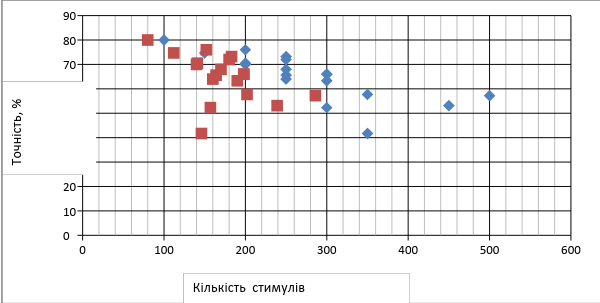
\includegraphics[width=\linewidth]{data3_irs13_total}}
	\\
	\subbottom[Розподіл за таблицею \ref{tbl:data3_irs24_total} \label{img:data3_irs24_total}]{%
		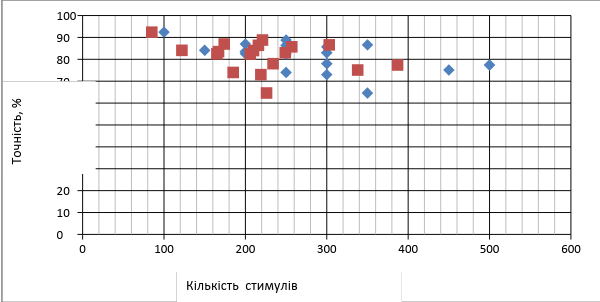
\includegraphics[width=\linewidth]{data3_irs24_total}}
	\caption{Розподіл точності розпізнання при відповідних стимулах: розпізнаних (червоні) та загальної кількості (сині) при апробації засобів формалізації голосової інформації в системах диспетчерського контролю за рухом автотранспорту для даних}
	\label{img:data3_irs}
\end{figure}

Порівнюючи дані розподілів, що приведені на рис. \ref{img:data1_irs} та \ref{img:data3_irs} можемо твердити про те, що з підвищенням загальної кількості стимулів відбувається зріст розпізнаних стимулів, що призводить до збільшення точності розпізнання при апробації засобів формалізації голосової інформації в системах диспетчерського контролю за рухом автотранспорту.

Моделювання рефлекторними системами при апробації засобів формалізації голосової інформації в системах диспетчерського контролю за рухом автотранспорту у цілому так і не дало результату, а для одного контексту дало близько 80\% точності (табл. \ref{tbl:data3_irs13_total}, \ref{tbl:data3_irs24_total} та рис. \ref{img:data3_irs}). Моделювання нейронною мережею майже не дало приросту в розпізнаванні, що свідчить про ефективність навчання згорткових фільтрів порівняно з попередньою обробкою.

\section*{Висновки до розділу 4}
\addcontentsline{toc}{section}{Висновки до розділу 4}

У розділі досліджені засоби формалізації голосової інформації в системах диспетчерського контролю за рухом автотранспорту.

При цьому, розглянуті особливості використання розроблених засобів формалізації голосової інформації в системах диспетчерського контролю за рухом автотранспорту показали, що для водія автомобілю, який буде здійснювати доставку продукції в процесі дистрибуції і вперше зіштовхнеться з засобом формалізації голосової інформації, що діє в рамках системи диспетчерського контролю за рухом автотранспорту, буде необхідно навчити систему розпізнавати його особистий голос з відповідним контекстом. Розроблений засіб формалізації голосової інформації дозволяє водію не відволікатись від управління автомобілем і слідкувати за дорожніми умовами та обстановкою, що дає змогу прискорити доставку продукції в процесі дистрибуції, а також забезпечити і підвищити рівень безпеки.

Проведена апробація засобів формалізації голосової інформації в системах диспетчерського контролю за рухом автотранспорту відбувалась за допомогою 4 пристроїв, 23 дикторів (11 жінок, 12 чоловіків), 94 варіантами стимулів (64 на основні реакції), 3046 зразків, додатково було прийнято 23 варіанти стимулів та 465 голосових зразків для реакції розпізнавання часу.

На декількох етапах досліджень рефлекторними системами як у цілому так і за контекстами не дало результатів. Точність під час навчання ЗНМ, на навчальних даних досягала 100\% і, відповідно, свідчило про перенавчання системи. Тому, далі, висунуто гіпотезу про недостатню кількість вхідних даних. У результаті було зібрано додаткові голосові дані для одного контексту: 1 пристрій, 1 диктор (чоловік), 925 варіантів стимулів, 3 реакції у контексті, 938 зразків, що призвело при моделюванні рефлекторними системами для одного контексту з великою вибіркою даних – до отримання точності не більше 70\%, а при ЗНМ – отримано точність більше 90\%.

Дослідження на цьому не були припинені, а, знову, була висунута наступна гіпотеза про недостатню якість вхідних голосових даних: втраті деяких діапазонів частот при записі на мобільному пристрої та погано вплинуло на роботу фонемного стенографа. Вирішено було зібрати додаткові голосові дані на ПК за допомогою якісного USB мікрофона і з використанням функції запису додатку фонемного стенографа, як і в оригінальній роботі: 1 пристрій, 1 диктор (чоловік), 350 варіантів стимулів, 64 реакції, 3200 зразків. Результати досліджень при апробації засобів формалізації голосової інформації в системах диспетчерського контролю за рухом автотранспорту показали те, що з підвищенням загальної кількості стимулів відбувається зріст розпізнаних стимулів, що призводить до збільшення точності розпізнання.

Підсумовуючи результати досліджень, можна стверджувати, що моделювання рефлекторними системами при апробації засобів формалізації голосової інформації в системах диспетчерського контролю за рухом автотранспорту у цілому так і не дало результату, а для одного контексту дало близько 80\% точності. Моделювання ЗНМ майже не дало приросту в розпізнаванні, що свідчить про ефективність навчання згорткових фільтрів порівняно з попередньою обробкою. Можна припустити що таке навчання не тільки знижує вимоги до вхідного звукового сигналу, а й у випадку низької якості звукових даних здатне відновити дані частково втрачені на етапі фонемного стенографа.
